\documentclass[10pt]{article}
\usepackage{pictex,amsmath,amssymb,amsfonts,amsthm,verbatim}
\usepackage{graphics,graphicx}
\usepackage{fullpage}
\usepackage{multirow}
\usepackage{gensymb}
\usepackage{mathrsfs}
\usepackage[version=4]{mhchem}
\usepackage{xcolor}
\usepackage{titlesec}
\usepackage{mdframed}
\usepackage[utf8]{vietnam}

\newmdenv[linecolor=red,skipabove=\topsep.skipbelow=\topsep,leftmargin=5pt,rightmargin=-5pt,innerleftmargin=5pt,innerrightmargin=5pt]{mybox}

\setlength{\voffset}{-0.25in}
\setlength{\headsep}{+0.5in}
\setlength{\parskip}{1em}
\setlength{\parindent}{0em}

\def\vu{\mathbf{u}}
\def\vs{\mathbf{s}}
\def\vv{\mathbf{v}}
\def\vw{\mathbf{w}}
\def\vb{\mathbf{b}}

\renewcommand{\implies}{\rightarrow}
\renewcommand{\lor}{\vee}
\renewcommand{\land}{wedge}
\renewcommand{\iff}{\leffrightarrow}
\newcommand{\TRUE}{\mathbf{T}}
\newcommand{\FALSE}{\mathbf{F}}
\newcommand{\universe}{\mathcal{U}}

\begin{document}
\begin{center}
	\textbf{THERMOCHEMISTRY}
\end{center}
\begin{enumerate}
	%1
	\item \textbf{Enthalpy of Chemical Reaction}\\
	\begin{mybox}
	\begin{center}
	$H = E + PV$
	\end{center}
	\end{mybox}
	The change in Enthalpy:
	\begin{mybox}
	\begin{center}
	$\Delta H = \Delta E + \Delta (PV)$
	\end{center}
	\end{mybox}
	If the pressure is held constant:
	\begin{center}
	$\Delta H = \Delta E + P \Delta V$
	\end{center}
	\textbf{Enthalpy of Reaction}\\
	- Because most reactions are constant-pressure process, we can equate the heat change in these cases to the change in enthalpy.
	\begin{center}
	\ce{ reaction -> products}
	\end{center}
	$\rightarrow{\mbox{The change in enthalpy, called the \textbf{Enthalpy of Reaction,$\Delta H$}}}$.\\
	\begin{mybox}
	\begin{center}
	$\Delta H = H(products) - H(reactants)$
	\end{center}
	\end{mybox}
	\begin{itemize}
		\item $\Delta H >0$, the reaction is an endothermic process.
		\item $\Delta H < 0$, the reaction is an exorthermic process.
	\end{itemize}
	\textbf{Thermochemical Equations}\\
	\ce{H2O(s) -> H2O(l)}\\
	$\Delta$ H = 6.01 kJ/mol.\\
	\textbf{A comparison of $\Delta H$ and $\Delta E$:}
	%2
	\item \textbf{The change of internal energy:}
	\begin{center}
	\begin{align}
    \Delta E = \Delta H - P \Delta V \\
    \Delta E = \Delta H - \Delta (PV)\\
             = \Delta H - \Delta (nRT)\\
             = \Delta H - RT \Delta n
    \end{align}         
	\end{center}
	For:
	\begin{itemize}
		\item $\Delta n = \displaystyle \Sigma n_{product} - \Sigma n_{reaction}$
		\item R = 8.314 J/mol $\cdot K$
		\item R = 0.08214 L $\cdot atm/mol \cdot K$
	\end{itemize}	
	%3
	\item \textbf{Enthalpy of Formation} ($\Delta H \degree$)\\
	\ce{aA + bB -> cC + dD}\\
	\textbf{Hess's law}\\
	- When reaction are converted to products, the change in enthalpy is the \textbf{same} wheither the reaction takes place in one step or in the series of steps.$\Delta H$ \textbf{depends} only on the \textbf{initial} and \textbf{final state}.\\
	- We have a reaction:\\
	\begin{center}
	\begin{align}
	\ce{CO(g) + \dfrac{1}{2} O2(g) -> CO2(g)}\\
	\Delta H = -283.0 kJ/mol\\
	\mbox{Then we inverse the equation:}\\
	\ce{CO2(g) -> CO(g) + \dfrac{1}{2} O2(g)}\\
	\Delta H = \textbf{+} 283.0 kJ/mol.
	\end{align}
	\end{center}
	Example:\\
	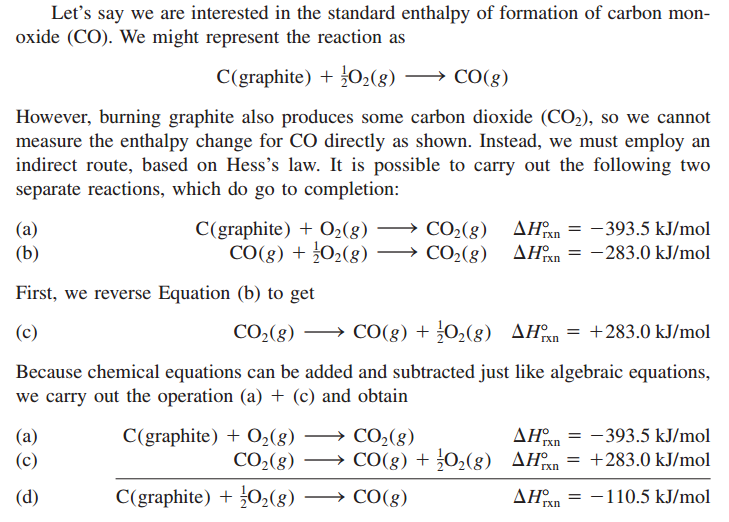
\includegraphics{hinh}
	%4
	\item \textbf{Entropy} (Phần quan trọng :))
	- The change in entropy of the system:
	\begin{mybox}
	\begin{center}
	$\Delta S_{sys} = \dfrac{q_{reversible}}{T}$
	\end{center}
	\end{mybox}
	The total change entropy is:
	\begin{center}
	$\Delta S = \Delta S_{surrounding} + \Delta S_{system}$
	\end{center}
	In reversible and irreversible process:
	\begin{itemize}
	\item Reversible Process: $\Delta S_{universe} = \Delta S_{system} + \Delta S_{surrounding} = 0$
	\item Irreversible Process $\Delta S_{universe} = \Delta S_{system} + \Delta S_{surrounding} > 0$
	\end{itemize}
	$\rightarrow{\mbox{The total entropy of the universe increases in any spontaneous process}}$\\
	\textbf{Some properties of the change in entropy:}
	\begin{itemize}
	\item \textbf{S} increases when \textbf{T} (temperature) increases
	\item when \textbf{M} increases then \textbf{S} increases.
	\end{itemize}
	And:
	\begin{mybox}
	\begin{center}
	$S_g \degree > S_l \degree > S_s \degree$
	\end{center}
	\end{mybox}
	Example:$F_2, Cl_2, Br_2, I_2$.\\
	$\rightarrow{S_{I_2} < S_{Br_2} < S_{F_2} < S_{Cl_2}}$  
\end{enumerate}
\end{document}	   		